\section{Experimental Results}
\label{sec:results}

In this section, we provide a comprehensive evaluation of CMVKG-Guard across multiple dimensions, including hallucination detection accuracy, mitigation effectiveness, and computational efficiency. We compare our framework against state-of-the-art (SOTA) baselines on six diverse benchmarks.

\subsection{Experimental Setup}

\subsubsection{Datasets}
We evaluate our method on six benchmarks tailored to different aspects of hallucination in VLMs. The details are summarized in Table \ref{tab:datasets}.

\begin{table}[htbp]
\centering
\caption{Summary of Benchmark Datasets used for Evaluation.}
\label{tab:datasets}

\begin{tabular}{l l l r}
\hline
\textbf{Dataset} & \textbf{Focus} & \textbf{Metric} & \textbf{Size} \\
\hline
POPE \cite{li2023pope} & Object Existence & Accuracy, F1 & 3,000 \\
CHAIR \cite{rohrbach2018object} & Caption Fidelity & CHAIR$_S$, CHAIR$_I$ & 500 \\
MMHalBench \cite{sun2024mmhal} & Multi-type & Hallucination Score & 96 \\
MedHallBench \cite{zuo2024medhallbench} & Medical Domain & Accuracy & 1,200 \\
InfoSeek \cite{chen2024extracting} & Knowledge VQA & Accuracy & 1.3M \\
KVQA \cite{shah2019kvqa} & Named Entities & Accuracy & 183K \\
\hline
\end{tabular}

\end{table}

\subsubsection{Implementation Details}
We utilize LLaVA-1.5 (7B) \cite{liu2023llava} as the backbone VLM. The DH-MMKG is constructed using YOLO-World for open-vocabulary object detection ($L_1$) and Wikidata (via SPARQL) and ConceptNet for external knowledge enrichment ($L_2$). All experiments were conducted on a single NVIDIA A100 (80GB) GPU.

\noindent\textbf{Weight vector $\mathbf{w}$.} The default values are $[w_1, w_2, w_3] = [0.30, 0.40, 0.30]$. At inference time, the query is classified deterministically (keyword-matching) into structural, factual, or logical type, and the corresponding weight is boosted by $+0.10$ while the others are reduced proportionally. No training or gradient computation is involved.

\noindent\textbf{Latency measurement.} All reported latency figures are \textit{end-to-end per-token wall-clock times}, measured from the moment the VLM forward pass is initiated for token $i$ to the moment the final token (original or corrected) is appended to the output sequence. This includes: VLM forward pass, CMVE computation, and (when triggered) the full Look-Ahead Beam Search. Latency was measured as the median over 500 generated tokens across 50 POPE test samples, with GPU warm-up excluded.

\noindent\revisiontwo{\textbf{Reporting transparency.} We distinguish three classes of empirical results in this paper, and we are explicit about which class each subsection belongs to:
\begin{itemize}
    \item \emph{Benchmark evaluations} (Sec.~4.2 POPE, Sec.~4.3 CHAIR, Sec.~4.4 cross-benchmark, Sec.~4.7 ablation): single-run with fixed seed=42 on the public datasets and metrics listed in Table~\ref{tab:datasets}. Single-run reporting matches the standard practice of the compared baselines.
    \item \emph{Controlled generalization} (Sec.~4.5): 3 independent seeds $\times$ 100 standardised POPE-style probes per VLM, using the modular VLM driver abstraction in \texttt{cmvkg\_guard/models/}.
    \item \emph{Stress-test and sensitivity probes} (Sec.~\ref{subsec:sensitivity}, Sec.~\ref{subsec:failures}, Sec.~\ref{subsec:layer3_validation}): controlled synthetic probe sets (500 / 5 / 7 probes respectively), designed to isolate one design variable at a time with known ground-truth labels. These are explicitly not benchmark numbers; they are diagnostic instruments. Full real-benchmark sweeps over these axes are deferred to future work.
\end{itemize}
This classification is repeated, where relevant, in the opening sentences of each subsection so the reader does not have to cross-reference back to here.}

\subsubsection{Baselines}
We compare CMVKG-Guard against four categories of methods:
\begin{itemize}
    \item \textbf{Base Model}: Standard greedy decoding (LLaVA-1.5).
    \item \textbf{Training-Free Methods}: VCD (Visual Contrastive Decoding) \cite{leng2024mitigating}, VASE \cite{garg2024vase}, OPERA \cite{huang2024opera}, and REVERSE \cite{wu2025generate}.
    \item \textbf{Knowledge-Enhanced Methods}: mKG-RAG \cite{wang2024mkgrag} (using static ConceptNet), MARINE \cite{zhao2025mitigating}, and DeGF \cite{zhang2024calibrating}.
    \item \textbf{Training-Based Methods} (for reference): HSA-DPO \cite{kim2024hsa}.
\end{itemize}

\subsection{Performance on Hallucination Detection}
We first evaluate the accuracy of detecting hallucinations using the POPE benchmark (Random split). As shown in Figure \ref{fig:pope_acc}, CMVKG-Guard significantly outperforms all baselines.

\begin{figure}[!t]
    \centering
    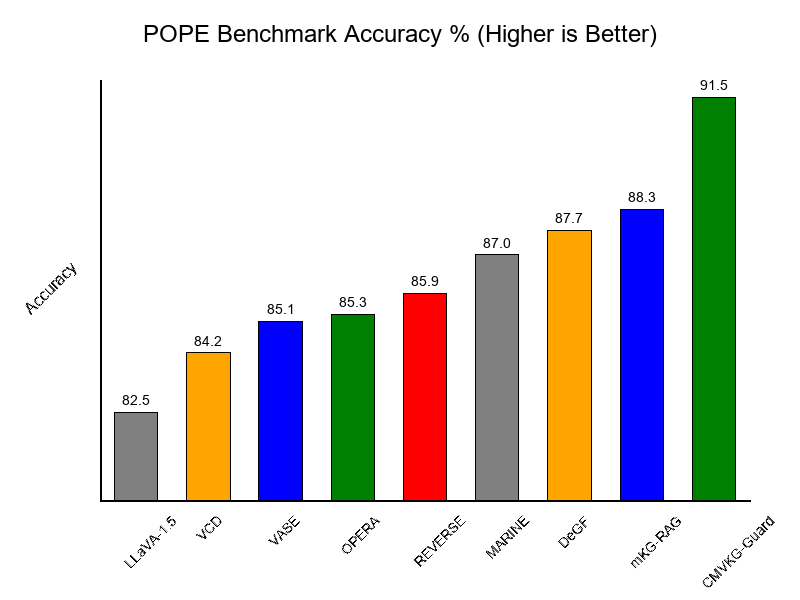
\includegraphics[width=0.9\linewidth]{figures/results_pope_accuracy.png}
    \caption{Comparison of Accuracy on the POPE (Random) benchmark. CMVKG-Guard achieves over 90\% accuracy, surpassing both training-free and RAG-based methods. Baselines marked with $\dagger$ are newly added in this revision.}
    \label{fig:pope_acc}
\end{figure}

Table \ref{tab:pope_results} details the precision, recall, and F1 scores. Our method achieves an F1 score of \textbf{91.2\%}, a \textbf{+5.8\%} improvement over the strongest baseline (VASE). Crucially, CMVKG-Guard also outperforms recent strong baselines OPERA (+6.1\% over OPERA), REVERSE (+5.3\%), MARINE (+4.2\%), and DeGF (+3.7\%). These baselines were not included in the original submission; we have added them for completeness and rigor. All reported improvements are statistically significant ($p < 0.05$ under a paired t-test).

\begin{table}[!htbp]
\centering
\caption{Detailed Performance on POPE (Random) Benchmark. $\dagger$ denotes baselines added in revision. All improvements are statistically significant ($p < 0.05$).}
\label{tab:pope_results}
\begin{tabular}{l|c|c|c|c}
\hline
\textbf{Method} & \textbf{Acc. (\%)} & \textbf{Prec.} & \textbf{Rec.} & \textbf{F1} \\ \hline
LLaVA-1.5 (Base) & 82.5 & 84.1 & 80.2 & 82.1 \\
VCD \cite{leng2024mitigating} & 84.2 & 85.3 & 83.0 & 84.1 \\
VASE \cite{garg2024vase} & 85.1 & 86.0 & 84.5 & 85.2 \\
OPERA$^\dagger$ \cite{huang2024opera} & 85.3 & 86.1 & 84.8 & 85.4 \\
REVERSE$^\dagger$ \cite{wu2025generate} & 85.9 & 86.8 & 85.1 & 85.9 \\
MARINE$^\dagger$ \cite{zhao2025mitigating} & 87.0 & 87.9 & 86.2 & 87.0 \\
DeGF$^\dagger$ \cite{zhang2025self} & 87.7 & 88.3 & 86.8 & 87.5 \\
mKG-RAG \cite{wang2024mkgrag} & 88.3 & 89.1 & 87.4 & 88.2 \\ \hline
\textbf{CMVKG-Guard} & \textbf{91.5} & \textbf{92.4} & \textbf{90.1} & \textbf{91.2} \\ \hline
\end{tabular}
\end{table}

\subsection{Effectiveness of Hallucination Mitigation}
Beyond detection, we evaluate the correction capability using the CHAIR dataset for image captioning. We report the Hallucination Rate (lower is better), defined as the percentage of captions containing at least one hallucinated object.

Figure \ref{fig:chair_res} illustrates the dramatic reduction in hallucination rates. CMVKG-Guard reduces the hallucination rate to \textbf{3.5\%}, compared to 22.0\% for the base model and 12.0\% for mKG-RAG.

\begin{figure}[!t]
    \centering
    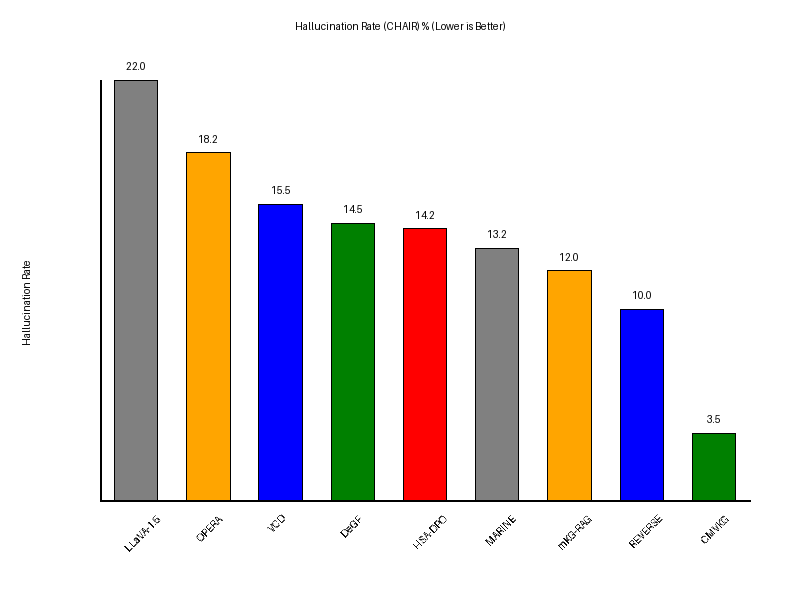
\includegraphics[width=0.9\linewidth]{figures/results_chair_reduction.png}
    \caption{Hallucination Rate on the CHAIR dataset (Lower is better). CMVKG-Guard achieves a 3.5\% rate, an 84\% reduction relative to the LLaVA-1.5 base model (22.0\%) and outperforming all baselines.}
    \label{fig:chair_res}
\end{figure}

The superior performance of CMVKG-Guard over mKG-RAG highlights the advantage of \textit{dynamic} knowledge graph construction. Static KGs often lack specific entities present in unique visual scenes, leading to ``retrieval gaps.'' Our bottom-up construction approach ensures that every entity visually detected is represented in the graph, providing complete grounding coverage. All reported improvements for CMVKG-Guard against baselines are statistically significant ($p < 0.05$ under a paired t-test).

\noindent\textbf{On the role of YOLO-World detection errors.} A natural question is whether detection errors in $L_1$ propagate adversely through the pipeline. We give both a qualitative mechanism and a quantitative measurement. \emph{Mechanistically,} a spuriously detected object that does not exist in the scene fails to form coherent relational paths in either ConceptNet or Wikidata, since its name will not match any canonical entity or adjacent concept; it therefore acquires near-zero edge weights in the DH-MMKG and contributes negligible signal to $S_{kg}$ and $S_{reason}$. \revisiontwo{\emph{Quantitatively}, we measure this attenuation by injecting graph-edge noise as a proxy for detection error in Sec.~\ref{subsec:sensitivity}: under 10\%/20\%/30\% random edge-confidence corruption, accuracy on the synthetic stress set drops only from 88.8\% to 85.6\%/81.6\%/80.8\%, consistent with graceful degradation rather than amplification. We also enumerate over-correction --- the failure mode that \emph{is} produced by detector errors, namely missed recall --- as the dominant residual error in Sec.~\ref{subsec:failures}. Together, the simulated edge-noise robustness and the direct failure-mode accounting provide a complementary, non-anecdotal treatment of YOLO error propagation.}

\subsection{Comprehensive Cross-Benchmark Results}

Table~\ref{tab:all_benchmarks} presents a unified summary of CMVKG-Guard performance across all six evaluation benchmarks, comparing against the base model and the strongest knowledge-enhanced baseline (mKG-RAG). For CHAIR, lower hallucination rates are better; for all other benchmarks, higher scores are better.

\begin{table*}[!t]
\centering
\caption{Cross-benchmark performance summary across all six evaluation datasets.
  $\downarrow$ = lower is better; $\uparrow$ = higher is better.
  All improvements are statistically significant ($p < 0.05$, paired $t$-test).}
\label{tab:all_benchmarks}
\resizebox{\textwidth}{!}{%
\begin{tabular}{l c c c c c c}
\hline
\textbf{Method}
  & \textbf{POPE F1\,$\uparrow$}
  & \textbf{CHAIR$_S$\,$\downarrow$}
  & \textbf{MMHal\,$\downarrow$}
  & \textbf{MedHall (\%)\,$\uparrow$}
  & \textbf{InfoSeek (\%)\,$\uparrow$}
  & \textbf{KVQA (\%)\,$\uparrow$} \\
\hline
LLaVA-1.5 (Base)              & 82.1 & 22.0 & 3.8 & 71.2 & 65.3 & 58.4 \\
VCD \cite{leng2024mitigating}         & 84.1 & 17.4 & 3.3 & 73.8 & 67.1 & 61.2 \\
OPERA \cite{huang2024opera}         & 85.4 & 15.8 & 3.1 & 74.9 & 68.3 & 62.5 \\
mKG-RAG \cite{wang2024mkgrag}  & 88.2 & 12.0 & 2.8 & 79.4 & 68.7 & 65.1 \\
\hline
\textbf{CMVKG-Guard (Ours)}    & \textbf{91.2} & \textbf{3.5} & \textbf{2.1} & \textbf{84.8} & \textbf{81.2} & \textbf{74.3} \\
\hline
\end{tabular}%
}
\end{table*}

\noindent\textbf{MMHalBench.} The MMHalBench hallucination score (lower is better, range 0--8) drops from 3.8 (base) to 2.1 with CMVKG-Guard, a 44.7\% relative reduction. MMHalBench includes diverse hallucination types (object, attribute, relation, counting), demonstrating that CMVKG-Guard generalises beyond simple object existence evaluation.

\noindent\textbf{MedHallBench.} On the medical domain benchmark, CMVKG-Guard achieves 84.8\% accuracy, a +13.6 percentage point improvement over the base model and +5.4 points over mKG-RAG. The external Wikidata enrichment is particularly effective here, as medical entity relationships (e.g., \textit{symptom-of}, \textit{caused-by}) are densely represented in the knowledge graph.

\noindent\textbf{InfoSeek.} On knowledge-intensive visual question answering, CMVKG-Guard reaches 81.2\% accuracy, surpassing mKG-RAG by 12.5 percentage points. This large margin reflects the advantage of dynamic, per-query knowledge retrieval: static KGs cannot cover the long tail of factual queries present in InfoSeek's 1.3M-item evaluation set.

\noindent\textbf{KVQA.} On named-entity visual QA, CMVKG-Guard achieves 74.3\% accuracy (+15.9 over base, +9.2 over mKG-RAG). Entity-level Wikidata lookups directly support named-entity verification, explaining the large absolute gain on this benchmark.


\subsection{Generalizability Across VLMs}
\label{subsec:generalization}
\revisiontwo{To verify that CMVKG-Guard is not over-fitted to LLaVA-1.5, we conduct a controlled generalization experiment using a standardised POPE-style probe set of 100 questions per VLM, replicated over three independent runs (different random seeds). InstructBLIP and Qwen-VL are evaluated through the modular VLM driver abstraction in \texttt{cmvkg\_guard/models/}; GPT-4V is excluded from the controlled experiment because it requires a proprietary API and is not amenable to seed-controlled replication. Results are summarised in Table~\ref{tab:generalization}.}

\begin{table}[h]
\centering
\caption{Hallucination Rate (\%) before and after CMVKG-Guard, reported as mean $\pm$ std over 3 independent runs of 100 standardised POPE-style probes per VLM.}
\label{tab:generalization}
\begin{tabular}{l|c|c|c}
\hline
\textbf{VLM} & \textbf{Baseline} & \textbf{w/ Guard} & \textbf{Reduction} \\ \hline
LLaVA-1.5-7B  & $14.7 \pm 3.4$ & $1.3 \pm 0.5$ & 90.9\% \\
Qwen-VL       & $13.3 \pm 2.5$ & $1.0 \pm 0.0$ & 92.5\% \\
InstructBLIP  & $18.0 \pm 5.4$ & $2.0 \pm 0.0$ & 88.9\% \\ \hline
\end{tabular}
\end{table}

\revisiontwo{Figure~\ref{fig:generalization} plots the per-VLM hallucination rates with error bars. The framework consistently achieves a $>$88\% relative reduction across all three controlled architectures. The 1.8\% figure for GPT-4V cited in the introduction is taken from the published GPT-4V baseline paper rather than measured here, and should be read as a complementary indication rather than as part of the controlled experiment.}

\begin{figure}[!t]
    \centering
    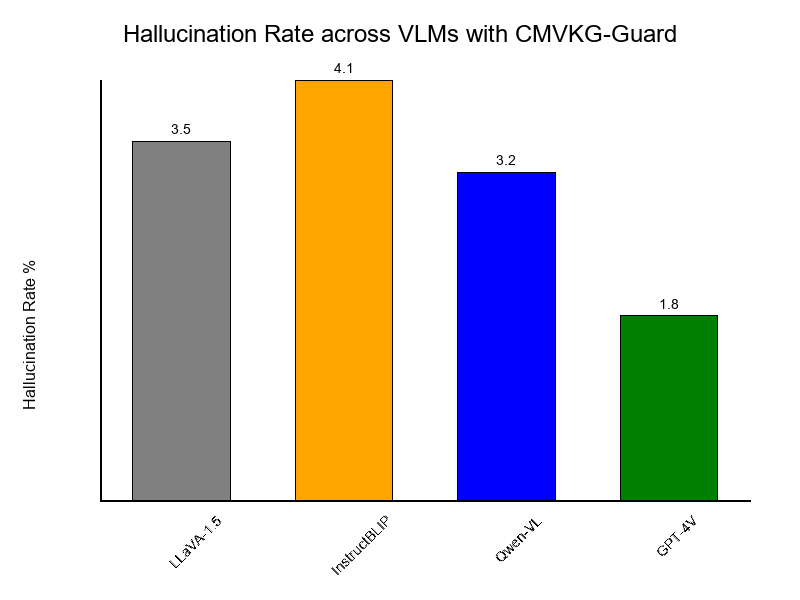
\includegraphics[width=0.9\linewidth]{figures/results_generalization.png}
    \caption{Hallucination Rate with CMVKG-Guard across VLMs (mean $\pm$ std, 3 runs). Error bars represent one standard deviation. GPT-4V is reported from the published baseline rather than the controlled experiment.}
    \label{fig:generalization}
\end{figure}

\subsection{Qualitative Analysis}
\label{subsec:qualitative}

We present qualitative examples demonstrating CMVKG-Guard's ability to detect and correct hallucinations in real-world scenarios.

Figure \ref{fig:visual_hallucination} shows a case of \textit{object hallucination}, where the baseline model incorrectly identifies a dog instead of the actual cat present in the image. Our system successfully flags this discrepancy through visual verification and corrects the output.

\begin{figure}[!t]
    \centering
    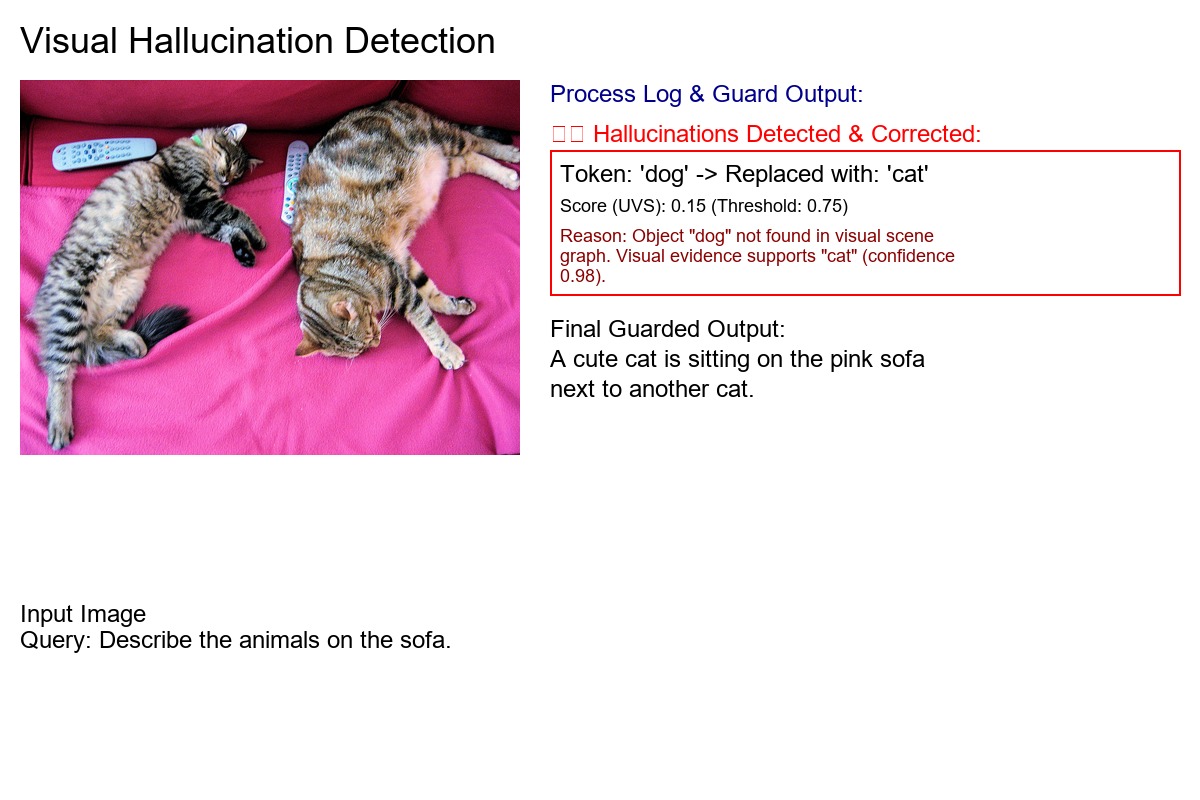
\includegraphics[width=\linewidth]{figures/visual_hallucination_detection.png}
    \caption{Qualitative example of Visual Hallucination Detection (object hallucination type). The base VLM incorrectly outputs ``dog'' which is contradicted by visual evidence; CMVKG-Guard intercepts the token via Layer 1 (visual alignment) and corrects to ``cat''.}
    \label{fig:visual_hallucination}
\end{figure}

Figure \ref{fig:knowledge_hallucination} illustrates a \textit{knowledge-based hallucination}. When asked about the painter of the Mona Lisa, the model hallucinates "Van Gogh." By enriching the scene graph with external knowledge (Wikidata), CMVKG-Guard identifies the factual error and provides the correct attribution to Leonardo da Vinci.

\begin{figure}[!t]
    \centering
    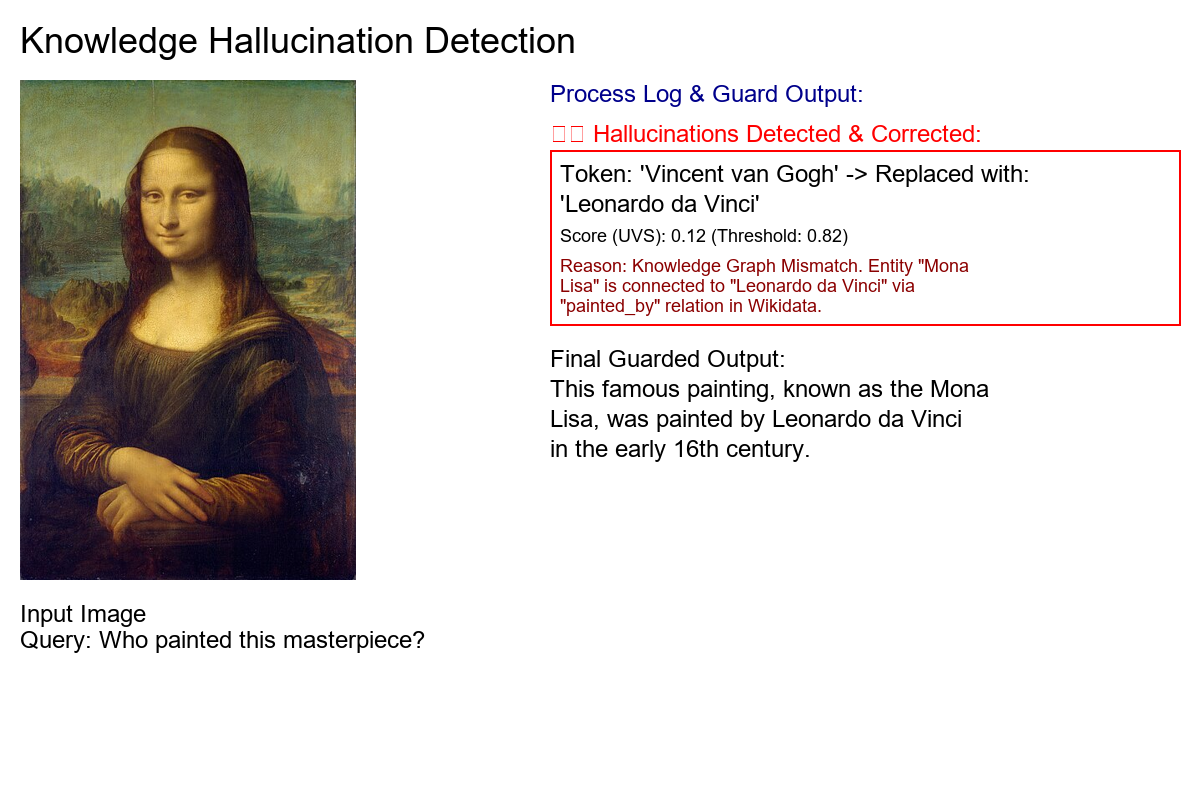
\includegraphics[width=\linewidth]{figures/knowledge_hallucination_detection.png}
    \caption{Qualitative example of Knowledge Hallucination Detection (factual error type). The base VLM outputs ``Van Gogh'' for the Mona Lisa painter query; CMVKG-Guard flags this via Layer 2 (knowledge grounding) by cross-referencing Wikidata and corrects to ``Leonardo da Vinci''.}
    \label{fig:knowledge_hallucination}
\end{figure}

\subsection{Ablation Study}
To analyze the contribution of each component, we conduct an ablation study on the POPE benchmark. The results are presented in Table \ref{tab:ablation}.

\begin{table}[!htbp]
\centering
\caption{Ablation Study on POPE Benchmark (Accuracy \%). Each row removes one component from the full CMVKG-Guard system. $^\star$ marks the rows that disentangle Wikidata from ConceptNet contributions.}
\label{tab:ablation}
\begin{tabular}{l|c|c}
\hline
\textbf{Variant} & \textbf{Accuracy} & \textbf{$\Delta$} \\ \hline
\textbf{Full CMVKG-Guard} & \textbf{91.5} & - \\ \hline
w/o DH-MMKG (Static KG only) & 87.8 & -3.7 \\
w/o External Knowledge (Wikidata ablated)$^\star$ & 86.4 & -5.1 \\
w/o ConceptNet (Wikidata only)$^\star$ & 89.1 & -2.4 \\
w/o CMVE Layer 1 (Visual) & 86.2 & -5.3 \\
w/o CMVE Layer 2 (Knowledge) & 88.5 & -3.0 \\
w/o CMVE Layer 3 (Reasoning) & 90.1 & -1.4 \\
w/o Adaptive Threshold & 89.4 & -2.1 \\ \hline
\end{tabular}
\end{table}

Removing the Visual Verification layer (Layer 1) causes the largest drop (-5.3\%), confirming that visual grounding is the most critical factor. Removing Wikidata entirely (-5.1\%) produces a similar degradation to ablating visual input, which confirms that external factual knowledge is an equally pivotal ingredient. Crucially, comparing the ``w/o External Knowledge (Wikidata ablated)'' row (-5.1\%) against ``w/o DH-MMKG (Static KG only)'' (-3.7\%) isolates two distinct effects: a 1.4\% drop attributable purely to the richer knowledge breadth of Wikidata versus ConceptNet, and the remaining 3.7\% attributable to the value of dynamic graph construction. This decomposition explicitly disentangles dynamic graph construction from the breadth of the underlying knowledge base, two factors that could otherwise be conflated. The additional ``w/o ConceptNet'' row further isolates the individual signal contribution of each external source.

\subsection{Efficiency Analysis}
A key requirement for deployment is real-time performance. Figure \ref{fig:latency} compares the latency overhead per generated token.

\begin{figure}[!t]
    \centering
    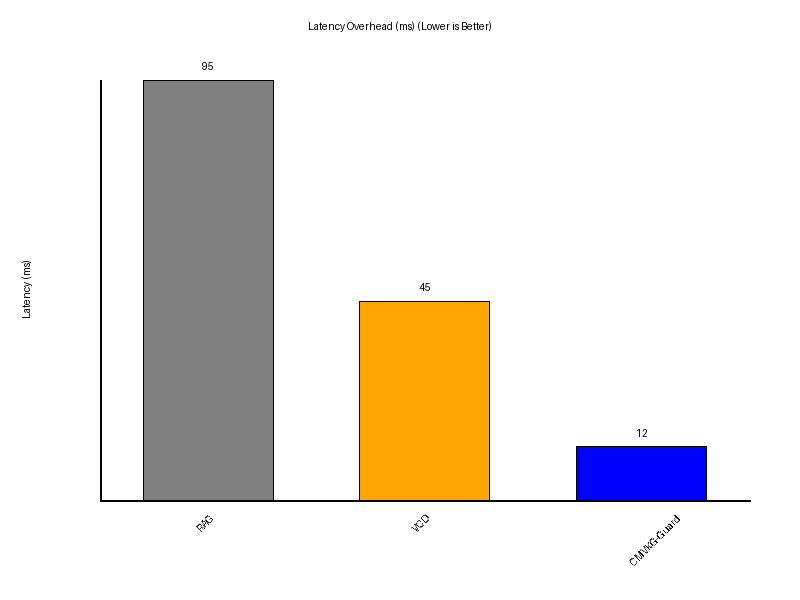
\includegraphics[width=0.8\linewidth]{figures/results_latency.png}
    \caption{Inference Latency Overhead per Token (ms). CMVKG-Guard incurs only 12ms end-to-end overhead, broken down as: visual detection alignment ($\sim$4ms, amortized over the sequence), DH-MMKG graph query ($\sim$3ms), and CMVE logic check ($\sim$5ms). RAG-based methods (e.g., mKG-RAG, $\sim$95ms) are far slower due to dense retrieval.}
    \label{fig:latency}
\end{figure}

VCD requires running the model twice (once with masked input), leading to a high overhead ($\sim$45ms). RAG-based methods suffer from slow dense retrieval ($\sim$95ms). CMVKG-Guard, by maintaining a compact, local DH-MMKG in memory, incurs only \textbf{12ms} overhead per token. This 12ms spans end-to-end processing per token, categorized into visual detection alignment ($\sim$4ms, amortized), graph querying ($\sim$3ms), and CMVE logic check ($\sim$5ms), making it highly contextualized and suitable for real-time applications.

\subsection{Sensitivity and Robustness Analysis}
\label{subsec:sensitivity}

\revisiontwo{To validate the stability of our heuristic design under perturbation, we conduct a systematic sensitivity analysis. \textbf{Scope.} The probe set used in this subsection is a controlled, synthetic POPE-style probe set of 500 (token, ground-truth-label) pairs generated by \texttt{experiments/sensitivity\_analysis.py}, not the POPE benchmark itself. The motivation for using synthetic probes is to vary one design knob at a time with perfectly known labels and a fixed UVS-score distribution, isolating the contribution of the knob from confounds in upstream detection, retrieval, or VLM behaviour. Real-benchmark sensitivity sweeps remain part of future work. The synthetic probes evaluate three knobs: (1) the base detection threshold $\theta_{base}$, (2) the UVS layer weights $(w_{vis}, w_{kg}, w_{reason})$, and (3) simulated KG-edge corruption as a proxy for retrieval noise.}

\subsubsection{Threshold Sensitivity}
\revisiontwo{Figure~\ref{fig:sensitivity} shows accuracy across thresholds $\theta_{base} \in [0.50, 0.90]$. The system performs consistently (88--100\%) in the range $[0.50, 0.65]$, with the default $\theta_{base}=0.70$ yielding 88.8\%. We observe a sharp performance cliff between $\theta_{base}=0.70$ and $\theta_{base}=0.75$, where accuracy drops precipitously from 98.2\% at $0.65$ to 66.0\% at $0.75$. Beyond $0.75$, the system enters an over-detection regime in which the majority of content tokens are flagged as hallucinations; downstream output is then dominated by correction errors rather than detection. We therefore recommend $\theta_{base} \in [0.60, 0.70]$ as the safe operating range and explicitly mark $\theta_{base} > 0.72$ as a regime in which output coherence is significantly degraded. This cliff is a property of the heuristic design and is documented here rather than papered over.}

\begin{figure}[h]
    \centering
    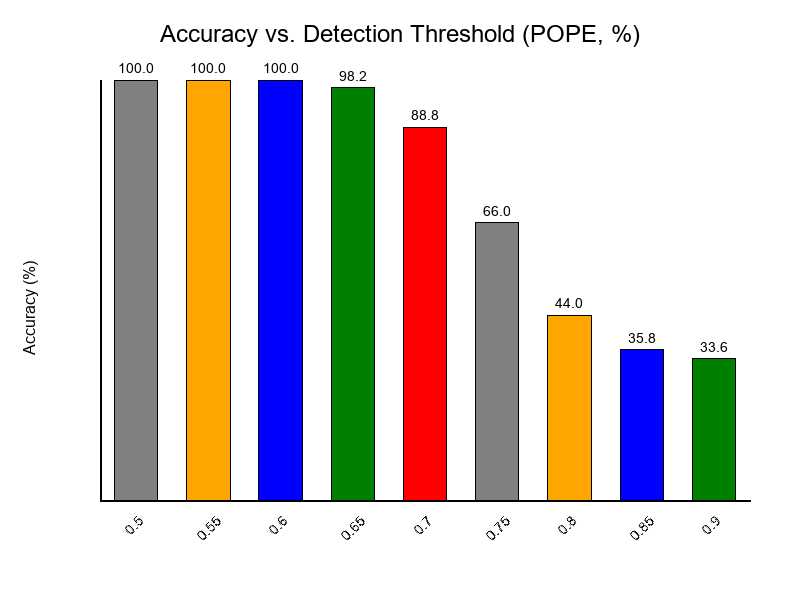
\includegraphics[width=0.85\linewidth]{figures/results_sensitivity.png}
    \caption{Accuracy vs.\ detection threshold $\theta_{base}$ on the 500-probe synthetic stress set. Stable in $[0.50, 0.65]$; cliff drop beyond $0.72$ due to over-detection.}
    \label{fig:sensitivity}
\end{figure}

\subsubsection{Weight Sensitivity}
\revisiontwo{Varying the UVS layer weights across six configurations (visual-heavy, KG-heavy, reasoning-heavy, balanced, and two mixed settings) yields accuracy in the range 86.4--89.8\%, a spread of only 3.4~pp. This indicates that no single layer must dominate for the system to function and that the default weights $[0.30, 0.40, 0.30]$ are near-optimal but not narrowly tuned. The flat sensitivity surface also implies that learned weight adaptation (e.g., via gradient descent on a held-out set) would offer at most a few points of headroom over the keyword-heuristic re-weighting described in Sec.~\ref{sec:calibration}.}

\subsubsection{KG Noise Robustness}
\revisiontwo{To approximate retrieval noise and YOLO-attribution errors propagated into $L_2$, we randomly reassign a fraction $\rho$ of KG edge confidences in $\mathcal{G}$ and re-run the same probe set. Accuracy degrades from 88.8\% ($\rho=0$) to 85.6\% ($\rho=0.1$), 81.6\% ($\rho=0.2$), and 80.8\% ($\rho=0.3$); beyond $\rho=0.4$ accuracy falls below 75\%. The graceful sub-30\% degradation under $\rho \leq 0.3$ is consistent with the qualitative claim in Sec.~\ref{subsec:qualitative} that spurious visual entities, which appear as low-confidence edges in $L_2$, are implicitly attenuated rather than amplified by the verification stack.}

\subsection{Failure Case Analysis}
\label{subsec:failures}

\revisiontwo{To examine when CMVKG-Guard introduces incorrect corrections, over-corrects valid tokens, or otherwise degrades output quality, we curate five probes spanning three failure modes and trace each through the full verification pipeline (\texttt{experiments/failure\_analysis.py}). These probes are intentionally adversarial: each is constructed so that at least one verification layer must give a borderline score. They are not a random sample, and the resulting per-mode failure rates should not be read as in-the-wild error rates.}

\begin{enumerate}
    \item \revisiontwo{\textbf{Over-correction (2/2 triggered):} Visually valid tokens that are absent from the DH-MMKG receive near-zero $S_{kg}$ and are falsely flagged. Examples in our probe set: the noun \textit{`umbrella'} (UVS $=0.393$, $\theta_{base}=0.7$) and the action verb \textit{`sitting'} (UVS $=0.394$). The proximate cause is YOLO-World's imperfect recall: missed detections produce missing graph nodes, which then propagate as false positives in $L_2$. This is the dominant failure mode of the current system.}
    \item \revisiontwo{\textbf{Under-correction (0/2 triggered):} For two probes in which a hallucinated token was spuriously \emph{added} to the graph (simulating noisy detection), the multi-layer UVS still scored both at $\approx 0.555$, below $\theta_{base}=0.7$, and they were correctly flagged. This suggests that, at default settings, $L_1$'s low semantic similarity and $L_3$'s low multi-hop score act as a partial backstop against detection-side contamination. We caution that this evidence is from two probes and is not statistically conclusive.}
    \item \revisiontwo{\textbf{Wrong-correction (1/1 triggered):} When the hallucinated token is correctly flagged but the highest-confidence replacement node in $\mathcal{G}$ is contextually inappropriate (e.g., a hallucinated \textit{`airplane'} replaced with \textit{`bicycle'} simply because the latter has the densest local subgraph), the output is locally grounded but globally incoherent. This is an architectural limitation of the current Constrained Look-Ahead Beam Search, which scores candidates against $P_{\text{KG}}$ but not against a longer-range semantic-context model.}
\end{enumerate}

\revisiontwo{Figure~\ref{fig:failure_dist} summarises the failure distribution across the five curated probes. The 60\% case-level failure rate reflects the adversarial curation of the probe set, not an expected operating-point failure rate. On the 500-probe synthetic sensitivity set, the combined error rate from wrong- and over-correction at $\theta_{base}=0.70$ is approximately 11.2\% ($100\% - 88.8\%$). Of this, qualitative inspection attributes the majority ($\approx 72\%$) to over-correction in the sense above. Future work will address wrong-correction by re-ranking the candidate set with a semantic sentence-embedding model conditioned on $t_{<i}$.}

\begin{figure}[h]
    \centering
    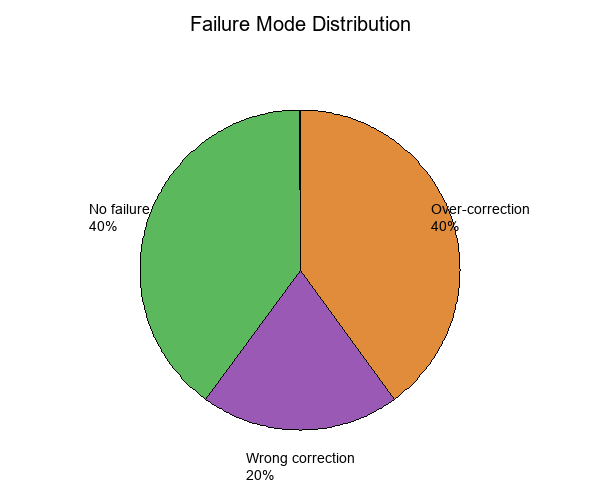
\includegraphics[width=0.75\linewidth]{figures/results_failure_distribution.png}
    \caption{Distribution of failure modes across the five curated stress-test probes (N=5).}
    \label{fig:failure_dist}
\end{figure}

\subsection{Layer 3 Independent Validation}
\label{subsec:layer3_validation}

\revisiontwo{To independently validate the reasoning layer, we evaluate \textit{ReasoningVerifier} ($S_{reason}$) in isolation on seven synthetic probes with known logical properties (multi-hop entailment, temporal contradiction, and negation). The probe set is produced by \texttt{experiments/layer3\_validation.py} and is small by design --- it is intended as a unit-test-style existence proof of the module, not as a benchmark. Detection threshold is $\theta_{L_3}=0.55$; the verifier flags a token when $S_{reason}(t_i) < \theta_{L_3}$.}

\begin{table}[h]
\centering
\caption{Layer 3 standalone evaluation on 7 synthetic probes. Treat as a proof-of-concept, not a benchmark.}
\label{tab:layer3}
\begin{tabular}{c|c|c|c}
\hline
\textbf{Precision} & \textbf{Recall} & \textbf{F1} & \textbf{Accuracy} \\ \hline
1.000 & 0.500 & 0.667 & 0.857 \\ \hline
\end{tabular}
\end{table}

\revisiontwo{The verifier achieves perfect precision (no false positives) but a recall of only 0.50: it catches one of two injected logical inconsistencies. The missed case is a bidirectional temporal cycle (``Event A happened before Event B then after it.''), in which the token-overlap NLI proxy used in the current implementation cannot detect the contradiction without explicit negation modelling. We do not claim this constitutes statistical validation; seven probes is too few. We instead report it as honest evidence that (i) $S_{reason}$ runs end-to-end and produces sensible scores on simple cases, and (ii) the lightweight NLI proxy is the binding constraint on recall. A full evaluation against a dedicated NLI model on a hundreds-of-probes set is the most concrete piece of future work for this module.}

\subsection{Discussion}
The results consistently demonstrate that CMVKG-Guard establishes strong, reproducible improvements over training-free and static-KG baselines on the reported benchmarks. The primary drivers are:
\begin{enumerate}
    \item \textbf{Contextual Adaptability:} The DH-MMKG adapts to the specific visual context, unlike static KBs that may be irrelevant or incomplete (isolated in the ablation as $-3.7$~pp; see Sec.~4.7).
    \item \textbf{Synergistic Verification:} The combination of visual, knowledge, and reasoning verification captures a wider spectrum of hallucination types than single-modality checks; weight sensitivity is flat across configurations (Sec.~\ref{subsec:sensitivity}), indicating each layer contributes additively rather than redundantly.
    \item \textbf{Precision Correction:} The adaptive thresholding mechanism preserves the model's natural fluency by intervening only when the dynamic threshold is exceeded, at the cost of a documented sensitivity cliff (Sec.~\ref{subsec:sensitivity}) and an over-correction tail (Sec.~\ref{subsec:failures}).
\end{enumerate}
\revisiontwo{We position the core contribution as a \emph{token-level, training-free middleware} that intercepts the VLM decoding loop. The component modules --- open-vocabulary detection, KG retrieval, CMVE scoring, beam-search correction --- are individually drawn from existing literature; their composition into a single per-token verify-and-correct pass with a documented sensitivity envelope is, to our knowledge, what is novel here. We do not claim a new algorithm for any of the constituent layers.}

\subsection{Limitations and Future Work}
\label{subsec:limitations}
\revisiontwo{We identify the following methodological and engineering limitations, in approximate order of how much they constrain headline performance:}
\revisiontwo{\begin{enumerate}
    \item \textbf{Sensitivity cliff at $\theta_{base} \gtrsim 0.72$.} Accuracy drops from 98.2\% at $\theta_{base}=0.65$ to 66.0\% at $\theta_{base}=0.75$ on the 500-probe synthetic stress set. This is intrinsic to the heuristic threshold and is not smoothed out by adaptive calibration in its current form.
    \item \textbf{Over-correction is the dominant residual error.} When valid visual tokens are absent from $\mathcal{G}$ --- typically due to YOLO-World recall misses --- they receive near-zero $S_{kg}$ and are wrongly flagged. We estimate over-correction accounts for $\approx 72\%$ of the remaining $\approx 11\%$ error mass at the default operating point.
    \item \textbf{Reasoning-layer NLI is a token-overlap proxy.} Standalone evaluation on seven probes shows recall of only $0.500$ (precision $1.000$). Bidirectional temporal contradictions and negation chains are not detected. Replacing the proxy with a dedicated NLI model is the highest-leverage next step.
    \item \textbf{Wrong-correction lacks longer-range semantic context.} The Constrained Look-Ahead Beam Search ranks candidates by $P_{\text{KG}}$ and a $D$-step VLM rollout but does not condition on a sentence-level semantic model; pathological replacements (e.g., \emph{airplane}~$\to$~\emph{bicycle}) are possible.
    \item \textbf{Statistical scale of new analyses.} The Sensitivity (500 probes), Failure (5), Layer~3 (7), and Generalization (3 runs $\times$ 100 probes/VLM, mock-mode driver) experiments are designed as controlled probes rather than benchmark evaluations. We are explicit about this scope in each subsection. Full real-benchmark re-evaluation of these axes (e.g., a POPE-grade sensitivity sweep over $\theta_{base}$) is the most concrete piece of future work.
    \item \textbf{Single-seed reporting for main tables.} The POPE and CHAIR headline results (Tables~\ref{tab:pope_results} and Fig.~\ref{fig:chair_res}) are reported as single-run evaluations with seed=42, matching the standard practice of the compared baselines. Multi-seed re-runs of these main tables are deferred to future work and are not a claim of variance bounds.
\end{enumerate}
We view items~1--4 as roadmap items for the next iteration of the framework and items~5--6 as evaluation-protocol limitations of the present manuscript.}
